\documentclass[aspectratio=169]{beamer}

\usepackage[ngerman]{babel}
\usepackage[utf8]{inputenc}
\usepackage[normalem]{ulem} %for strikeout and underline

% Themes, Colors, Fonts
\usetheme{csthm}
\usepackage{csjavalst}

\newcommand{\code}[1]{\textnormal{\lstinline|#1|}}
\newcommand{\enquote}[1]{\glqq{}#1\grqq{}}

% ======================== title page =========================
\author{Florian Maximilian Dörr, Hendrik Wagner}
\title[OOP]{II2021 Entwicklung eines autonomen Fahrzeugs}
\subtitle{Team 2}
\institute[THM]{Technische Hochschule Mittelhessen}
\titlegraphic{
	% \includegraphics[width=\paperwidth]{img/pawel-czerwinski-VhDgReMsz8w-unsplash.jpg}
	}
\date{13. Juli 2022}

% bildverarbeitung
	% transformation
    % Line Detection
	% m-gedöns
% autonomes fahren
	% pid-regelung steuerung
	% pid-regelung speed
	% evtl. noch Überholen?
	% state stack

% code kommentieren!
% alles so vorbereiten, dass wir leicht alles starten können und losfahren können

% ============================ begin document =================
\begin{document}
\newgeometry{left=3mm,right=3mm,top=0cm,bottom=.5cm}

\begin{frame}
	\titlepage
\end{frame}

\AtBeginSection[]
{
	\begin{frame}
		\frametitle{Inhalt}
		\tableofcontents[currentsection]
	\end{frame}
}


\section{Bildverarbeitung mit OpenCV}

\begin{frame}{Bildtransformation}
	\begin{center}
		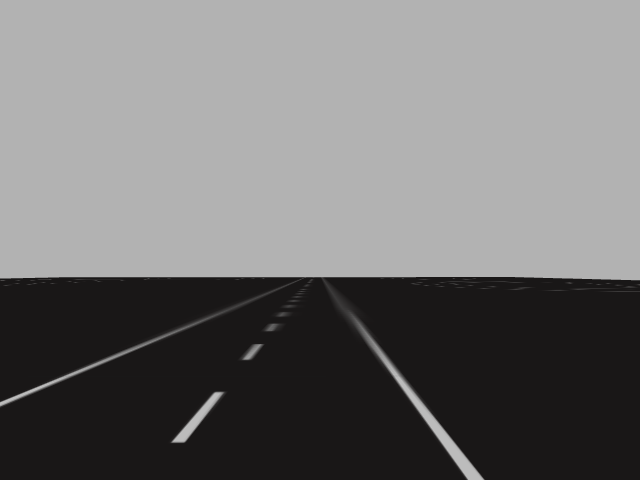
\includegraphics[width=.20\textwidth]{img/gerade_raw.png}
		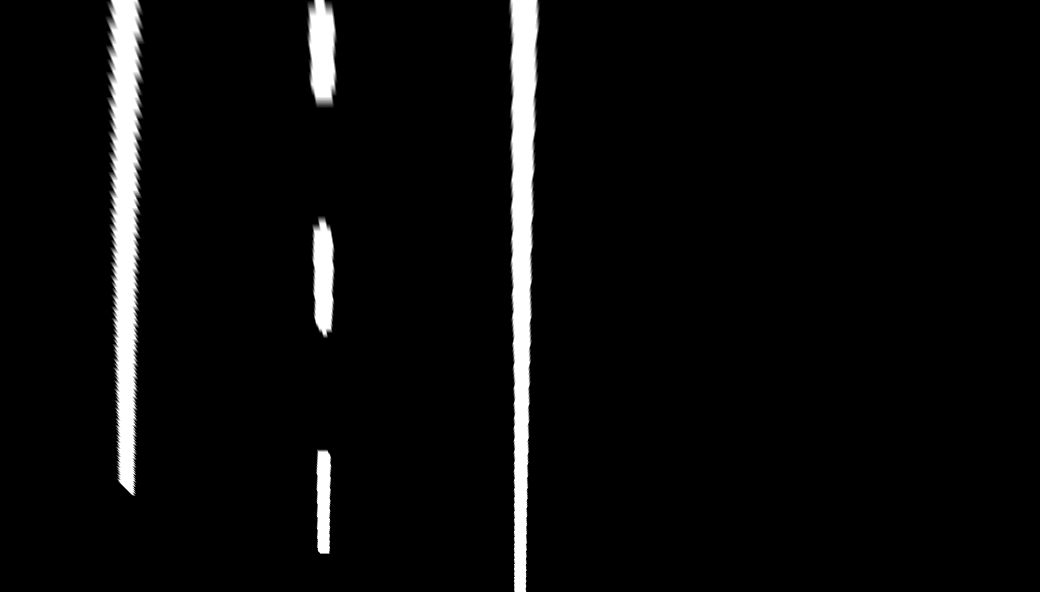
\includegraphics[width=.20\textwidth]{img/gerade_transformed.png}
	\end{center}
	\vspace{0.5em}
	\begin{center}
		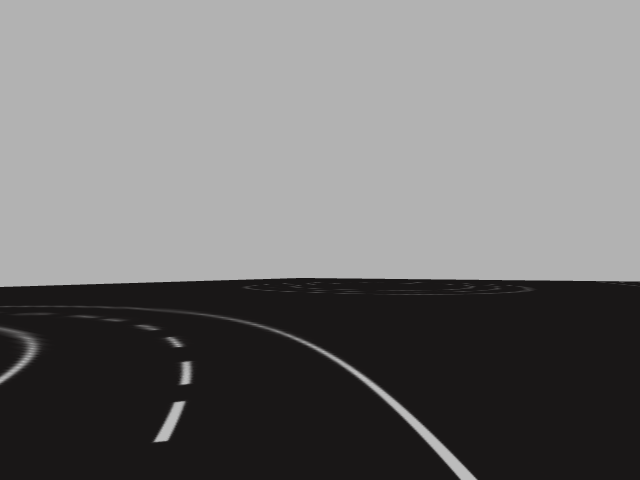
\includegraphics[width=.20\textwidth]{img/kurve_raw.png}
		
\includegraphics[width=.20\textwidth]{img/kurve_transformed.png}
	\end{center}
	% Bilder
	\begin{enumerate}
		\item Zuschnitt des Inputs auf die Region of Interest
		\item Ermittlung Kameraposition, FOV (\emph{Homographie}) für Testtransformationsmatrix
		\item Perspektivische Transformation mithilfe Zieltransformationsmatrix
	\end{enumerate}
\end{frame}

\begin{frame}{Linienerkennung | \enquote{Regions of interest}}
	\begin{itemize}
		\item Aufteilung des tranformierten Bildes in zwei Regionen
		\item Start in Bereich, in dem Anfang der Linie erwartet wird
		\item Es wird in festen Schritten, Punkte der Linie abgegangen $\rightarrow$ Auflösung frei wählbar (40 Punkte)
		\item Weiteres vorgehen abhängig, ob ein ein weißer Pixel gefunden wurde oder nicht:
		      \begin{enumerate}
			      \item Weißen Pixel gefunden: Punkt wird in Liste abgespeichert und nächster Suchbereich wird nach diesem Punkt in Verbindung mit dem letzen Punkt (Steigungstendenz) bestimmt
			      \item Kein Weißer Pixel gefunden: Der nächste Suchbereich ist der jetzige, er wird jedoch erweitert/aufgefächert
		      \end{enumerate}
	\end{itemize}
	\begin{center}
		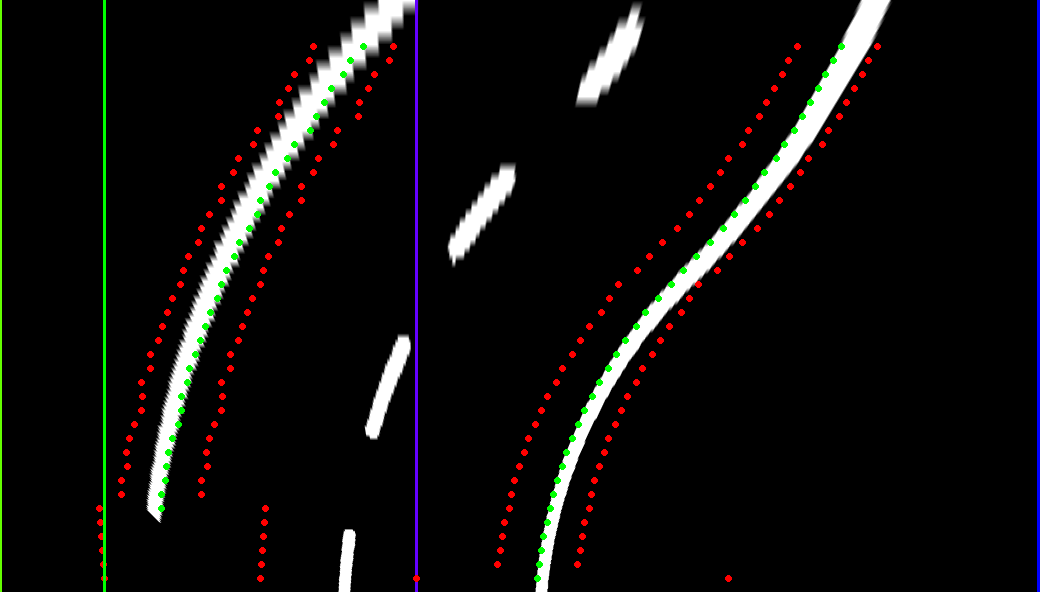
\includegraphics[width=.35\textwidth]{img/line_detection_normal.png}
		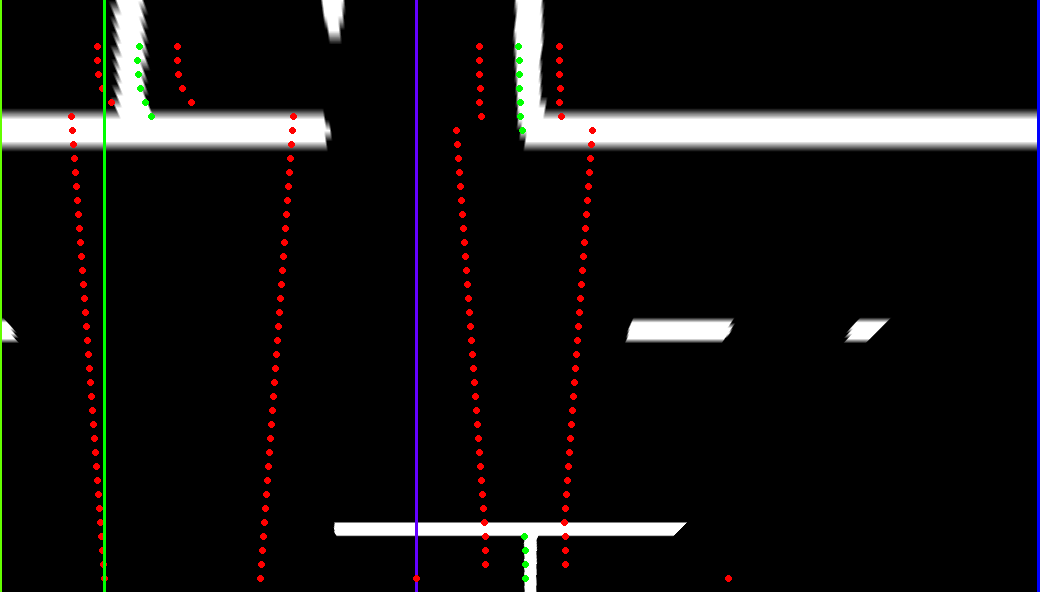
\includegraphics[width=.35\textwidth]{img/line_detection_crossing.png}
	\end{center}
\end{frame}

\begin{frame}{Linienerkennung | Steigungsermittlung}
	\begin{center}
		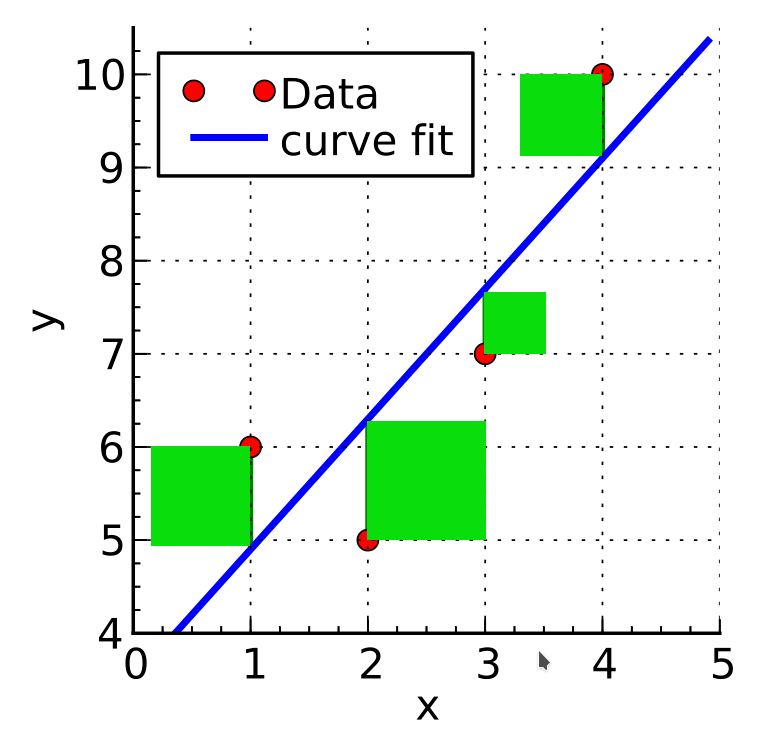
\includegraphics[width=.25\textwidth]{img/least_squared.png}
	\end{center}
	\begin{itemize}
		\item Bildung einer Gerade über die ermittelten Punkte mithilfe der \emph{Methode der kleinsten (Fehler-) Quadrate}
		      \begin{itemize}
			      \item Sucht eine Gerade, dessen quadrierter Distanz zu allen Punkten minimal ist
			      \item Resultiert in einen Steigungswert $m$, welcher für den Lenkwinkel und der Geschwindigkeit verwendet werden kann
			      \item Dank der Transformation ist die Soll-Steigung $m=0$!
		      \end{itemize}
	\end{itemize}
\end{frame}

\section{Autonomes Fahren}

\begin{frame}{PID | Lenkung}
	\begin{itemize}
		\item Lenkung wird mittels zwei PID-Reglern gesteuert
		      \begin{enumerate}
			      \item Kurven-Lenkung: $m$ Wert wird als Eingabe verwendet
			      \item Positionierung innerhalb der Fahrspur: Es existiert ein Sollwert für den ersten erkannten weißen Pixel, der eingehalten werden soll
		      \end{enumerate}
		\item Es werden nur $50\%$ der erkannten Punkte und die resultierende Steigung verwendet\\
		      \rotatebox[origin=c]{180}{$\Lsh$} Es ist hinderlich für die Lenkung zu weit in die \enquote{Zukunft} zu schauen
		\item Werte werden auf $45^\circ$ bzw. $-45^\circ$ beschränkt
		\item PIDs arbeiten \enquote{gegeneinander} $\rightarrow$ Kurven-Lenkung ist der \emph{dominante} Wert, Positionierung \emph{korrigierender} Wert
	\end{itemize}
\end{frame}

\begin{frame}{PID | Geschwindigkeit}
	\begin{itemize}
		\item PID-Regler für Geschwindigkeit in Abhängigkeit von vier Faktoren:
		      \begin{enumerate}
			      \item Die Steigung der ersten 50\% der erkannten Punkte (linke und rechte Linie)
			      \item Die Steigung der hinteren 50\% der erkannten Punkte (linke und rechte Linie) $\rightarrow$ hier ist eine Vorausschau sinnvoll und notwendig
		      \end{enumerate}
		\item Mindestens 2.55 $\frac{m}{s}$ (9.18 $\frac{km}{h}$), maximal 5.4 $\frac{m}{s}$ (19.44 $\frac{km}{h}$) im normalen Modus\\
		      \rotatebox[origin=c]{180}{$\Lsh$} Drosselung bei Überholmanöver (maximal 2.7 $\frac{m}{s}$)
	\end{itemize}
\end{frame}

\begin{frame}{Überholmanöver}
	\begin{itemize}
		\item Drosselung der Geschwindigkeit $3m$ vor einem Hindernis
		\item Spurwechsel $1.6m$ vor dem Hindernis\\
		      \rotatebox[origin=c]{180}{$\Lsh$} Soll-Werte für Lenkung-PIDs wechseln auf linke Linie
		\item Spurwechsel sobald rechts neben dem Auto keine Box detektiert wird\\
		      \rotatebox[origin=c]{180}{$\Lsh$} Soll-Werte für Lenkung-PIDs wechseln zurück auf die rechte Linie
		\item Problem: Region-of-Interests stimmen nicht mehr!\\
		      \rotatebox[origin=c]{180}{$\Lsh$} Verschieben der Region-of-Interests nach links nach erstem Wechsel und nach dem Zurückfahren wieder nach rechts
	\end{itemize}
\end{frame}

\begin{frame}{Einparkmanöver}
	\begin{enumerate}
		\item Parklücke suchen: Rechter Sensor sucht zwei Hindernisse in Folge
		\item Beim zweiten Hindernis abbremsen und Einparksequenz starten
		      \begin{enumerate}
			      \item Festgelegte Einlenkungswinkel beim Rückwärtsfahren
			      \item Optimierung der Position zwischen den Hindernissen $\rightarrow$ mittig
		      \end{enumerate}
		\item Nach kurzer Parkzeit wird die Ausparksequenz gestartet
		      \begin{enumerate}
			      \item Zurückfahren bis zum Wunschabstand zum hinteren Hindernis
			      \item Festgelegtes Ausparkverhalten und Reaktivierung des autonomen Fahrens
		      \end{enumerate}
	\end{enumerate}
	\begin{figure}
		{\small \caption{Skizziertes Einparkmanöver}}
		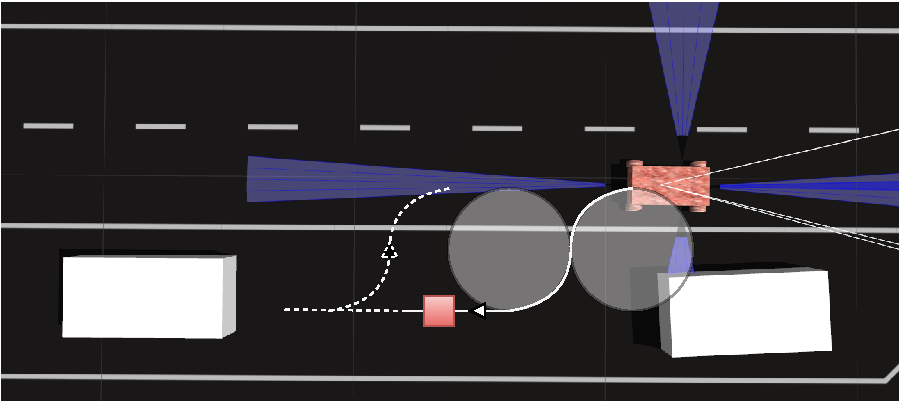
\includegraphics[width=.45\textwidth]{img/mett.drawio.pdf}
	\end{figure}
\end{frame}

\begin{frame}{\enquote{State-Machine} \& Remote Controller}
	\begin{itemize}
		\item Grundkonzept: Stack | durch \emph{pop} von einem Stack in den nächsten
		\item Zustände werden mithilfe eines Enums definiert
		\item Initialbelegung des Stacks mit allen gewünschten Fahrabschnitten, die sich ggf. selbst entfernen können
		\item Kommunikation mit State-Machine mithilfe vom Remote Controller
		      \begin{itemize}
			      \item \code{w, a, s, d}: Manuelles Fahren
			      \item \code{q} Remote Controller wird de/aktiviert, indem der entsprechende State oben drauf gelegt wird bzw. entfernt wird
			      \item \code{r} Zurücksetzen der PID-Werte
			      \item \code{x} Zurücksetzen der Zustandsmaschine durch \emph{clear} und erneute Belegung des Stacks
			      \item \code{p} Entfernung des obersten Zustands des Stacks
		      \end{itemize}
	\end{itemize}
\end{frame}

\begin{frame}{Speed Graph}
	\begin{center}
		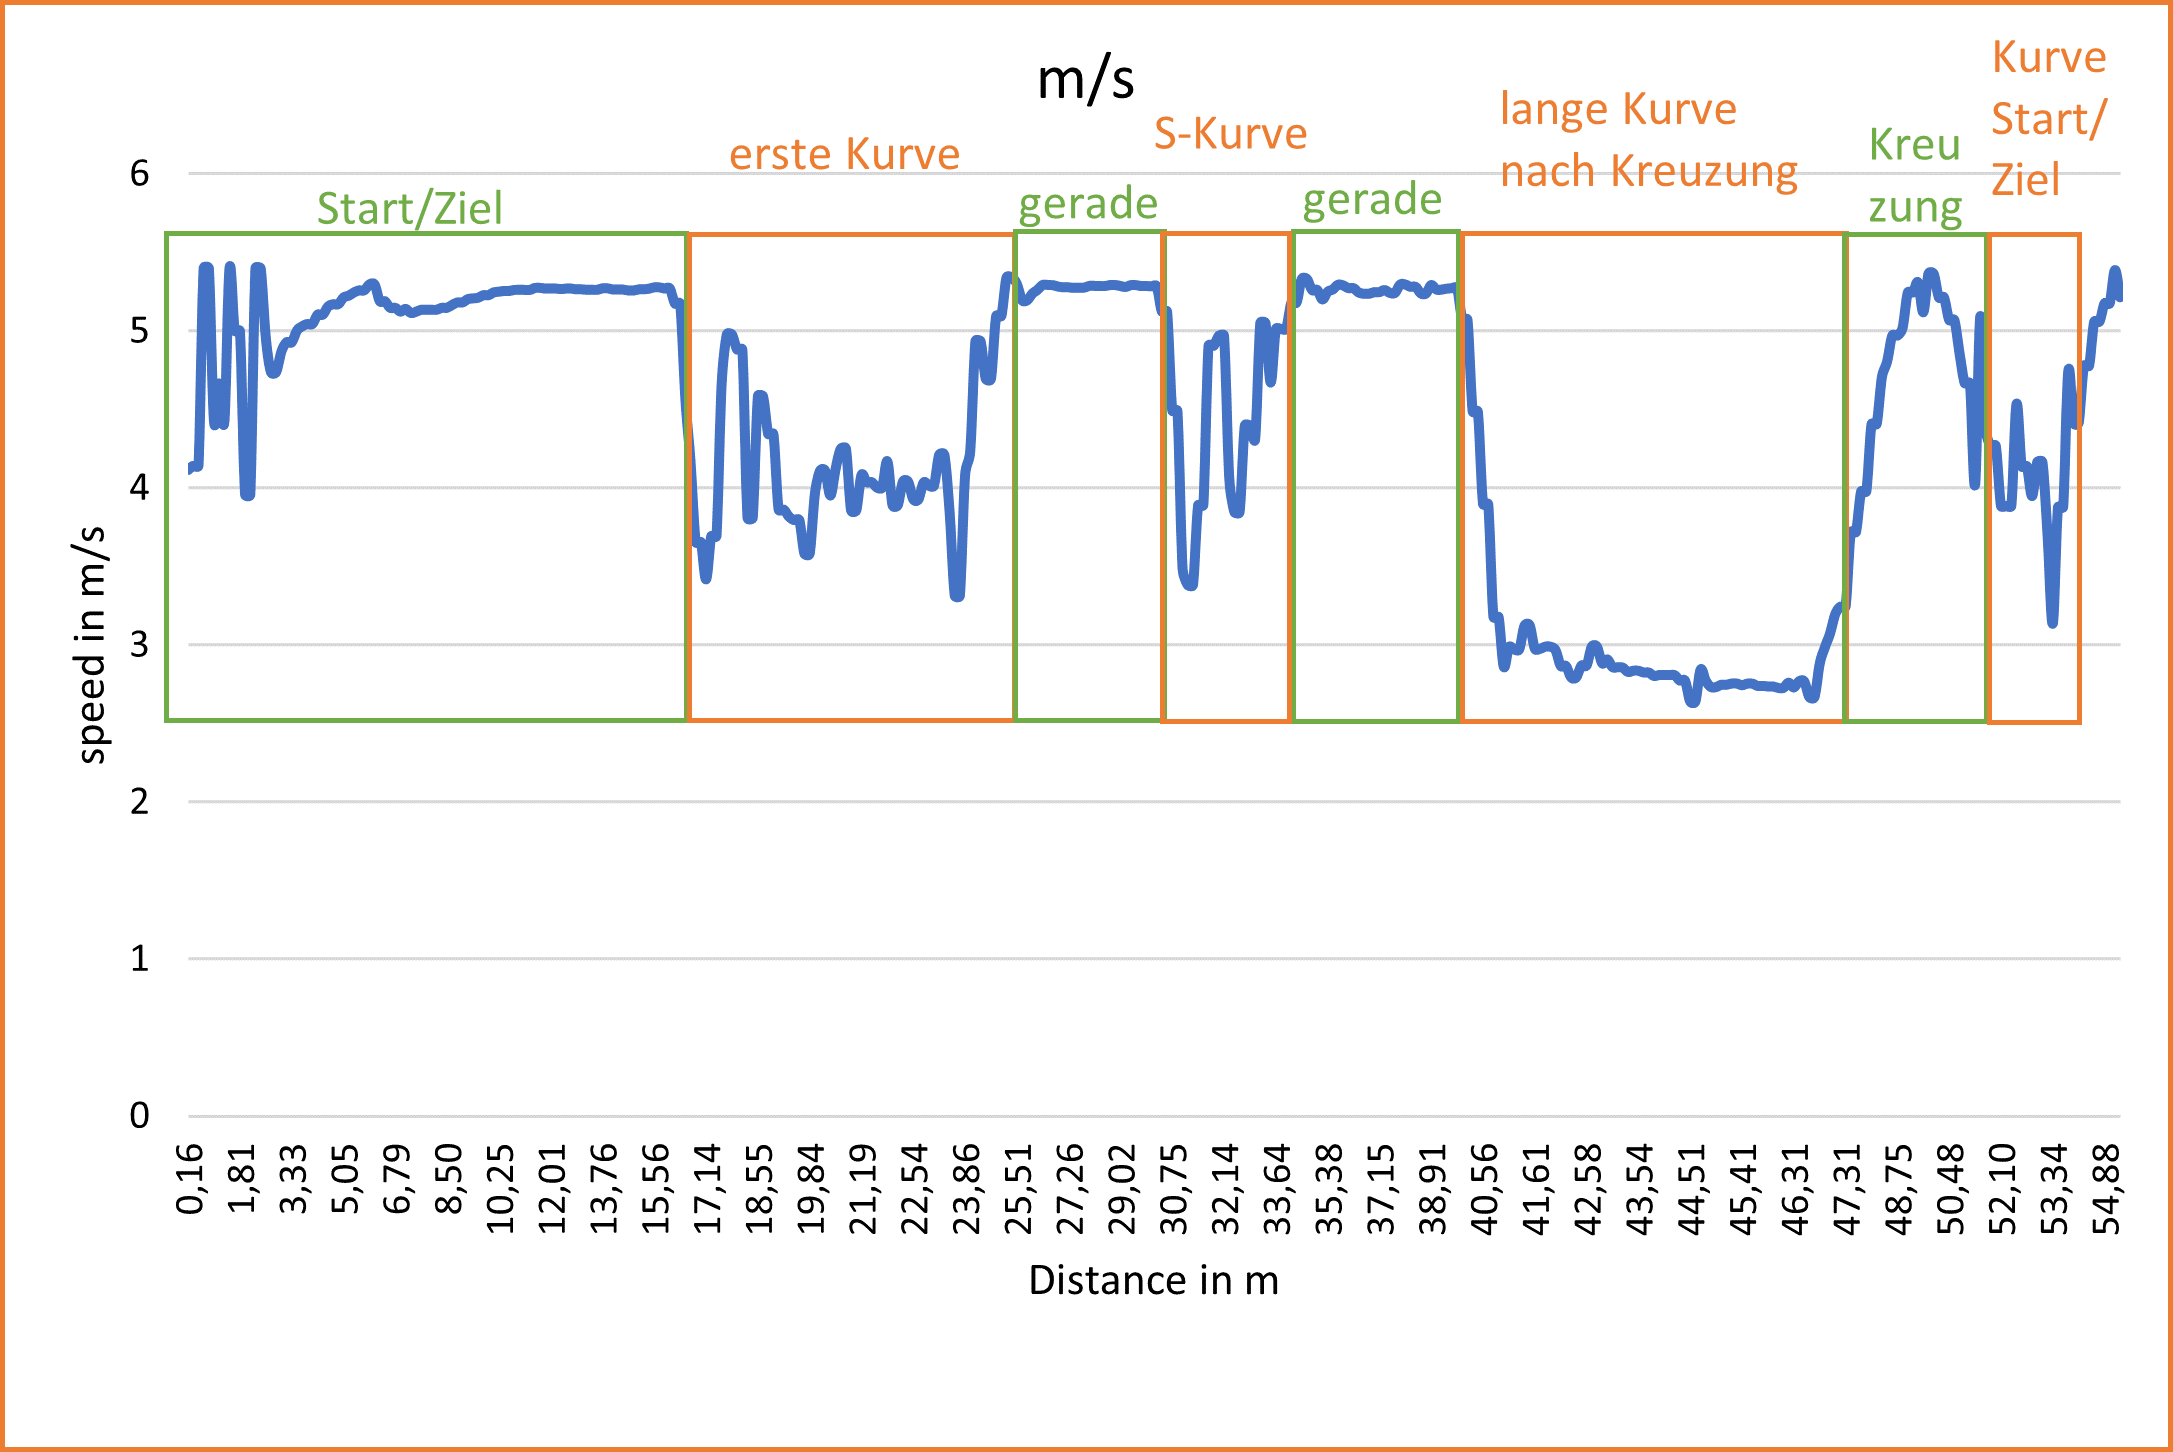
\includegraphics[height=.9\textheight]{img/SpeedPlot.png}
	\end{center}
\end{frame}

\begin{frame}[fragile]{Quellen}

	\begin{itemize}
		\item \emph{Least Squared Graph}: Krishnavedala, CC BY-SA 3.0 via Wikimedia Commons, modifiziert (Quadrate)
	\end{itemize}

\end{frame}


\end{document}